\documentclass[12pt]{article}
\usepackage[utf8]{inputenc}
\usepackage{amsmath,amssymb}
\usepackage[T2A]{fontenc}
\usepackage[russian]{babel}
\usepackage{graphicx}
\usepackage{subfigure}

\DeclareGraphicsExtensions{.pdf,.png,.jpg}
\usepackage{hyperref}
\usepackage{wrapfig}
\usepackage[left=20mm, top=20mm, right=10mm, bottom=20mm]{geometry}

\usepackage{amsmath} 
\usepackage{amsfonts} 
\usepackage{amssymb} 
\usepackage{wasysym} 
\usepackage{fancyhdr}
\usepackage{revsymb}

\usepackage[labelsep=period]{caption}

\pagestyle{fancy}
\fancyhf{}
\lhead{Семинар 2. Фотоэффект. Эффект Комптона}
\rhead{\textit{Клименок К.Л., МФТИ 2020}}
\rfoot{\thepage}


\begin{document} 

\title{\textbf{Семинар 2. Фотоэффект. Эффект Комптона}}
\author{\textbf{Клименок Кирилл Леонидович}}
\date{12.06.2020}
\maketitle

\section{Теоретическая часть}
В этом семинаре мы рассмотрим, как идея Планка из первого семинара о квантуемости энергии излучения оказалась применима при описании фотоэффекта, и посмотрим, как фотоны могут вести себя как частицы в эффекте Комптона.

\subsection{Внешний одноквантовый фотоэффект}
Не надо пугаться этого длинного названия --- это тоn обычный фотоэффект, о котором говорят еще в школе, но с некоторыми оговорками. <<Внешний>> означает, что электроны при освещении катода вылетают в вакуум лампы (в отличие от внутреннего фотоэффекта в полупроводниках, когда электрон остается внутри), а <<одноквантовый>> означает, что 1 квант света выбивает 1 электрон (возможна ситуация, когда несколько квантов света выбивают один электрон). Для начала, сформулируем все основные экспериментальные результаты по фотоэффекту, а после этого проанализируем их.

\begin{enumerate}
    \item Фототок появляется при облучении катода светом
    \item Максимальный фототок оказывается пропорционален интенсивности
    \item Фотоэффект происходит безинерционно, т.е. при включении света ток начинается сразу же, никакого времени для накопления энергии нет
    \item У фотоэффекта есть красная граница: если частота падающего света ниже нее, то фотоэффекта нет
    \item Максимальная энергия электронов зависит только от частоты падающего света
\end{enumerate}

\noindent
Давайте посмотрим на экспериментальные результаты по измерению вольт-амперной характеристики для фотоэлектронной лампы. Первая особенность состоит в том, что даже при отрицательном напряжении ток в лампе может идти. Это означает, что электроны, которые под действием света вылетают из катода, обладают достаточной кинетической энергией, чтобы преодолеть это напряжение. А напряжение, при котором ток прекращается, называется запирающим. При этом оказывается, что это запирающее напряжение зависит от частоты света, которым мы облучаем катод. То есть, неявно повторяется гипотеза Планка о том, что энергия излучения зависит от частоты. Вторая особенность связана с тем, что запирающее напряжение не зависит от интенсивности света. А от него зависит только фототок в стационарном режиме при большем разгоняющем напряжении.
\begin{figure}[h]
    \centering
    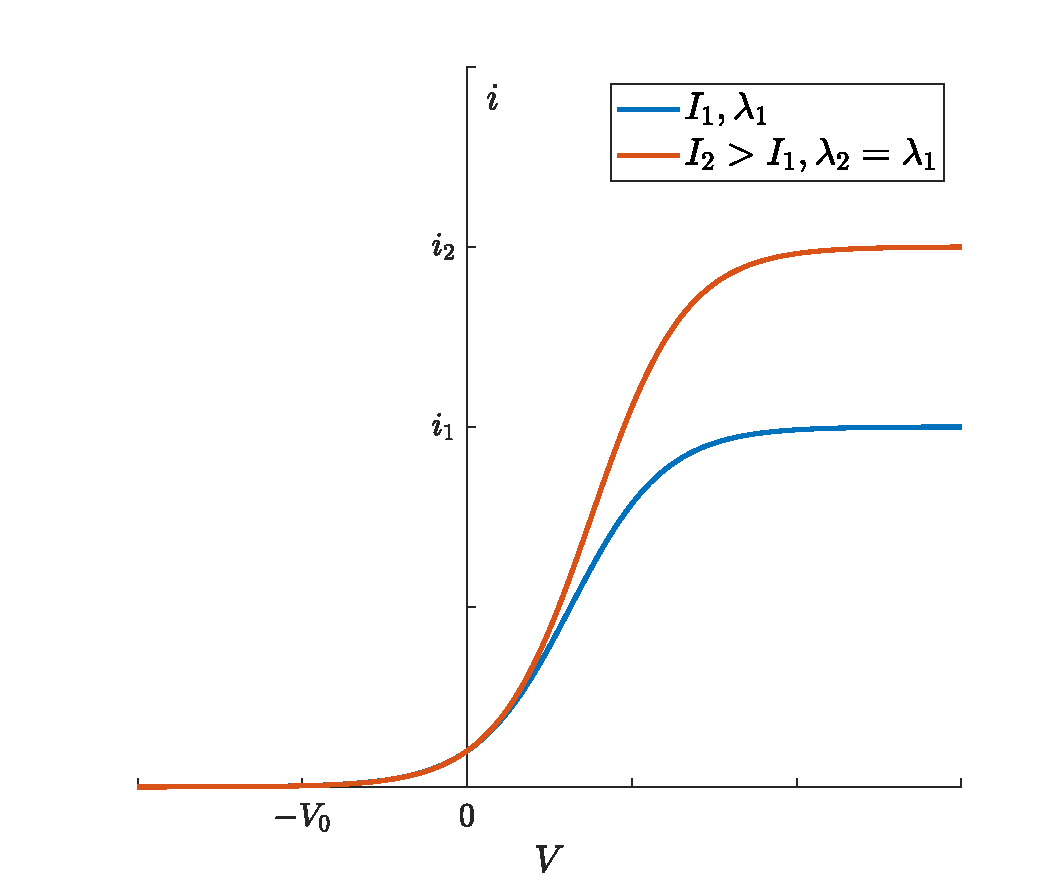
\includegraphics[width=0.8\textwidth,keepaspectratio]{Seminar_02/pics/pic_01.pdf}
    \caption{Вольт-амперная характеристика фотокатодной лампы для света одинаковой частоты и разной интенсивности}
    \label{fig:sem_02_photocatod_VAX}
\end{figure}

\noindent
Теперь, понимая все это, мы можем написать закон сохранения энергии для фотоэлектрона, или, как его принято называть, закон Эйнштейна для фотоэффекта:
\begin{equation}
    \hbar \omega = \dfrac{m_eV^2}{2} + A_{\text{вых}}
\end{equation}

\noindent$A_{\text{вых}}$ это работа выхода электрона из металла. Попытаемся объяснить, что она означает, с помощью рисунка \ref{fig:sem_02_electron_energy}. Примем за ноль энергию свободного покоящегося электрона. Поскольку из металла электроны не вылетают, то их энергия там отрицательна. Электроны, которые содержатся в металле, образуют целую зону по энергиям, и расстояние от вершины этой зоны до 0 и есть работа выхода. Если же энергия света больше, чем работа выхода, то выбитые электроны будут иметь энергии от нулевой до максимальной, рассчитанной по закону Эйнштейна.
\begin{figure}[h]
    \centering
    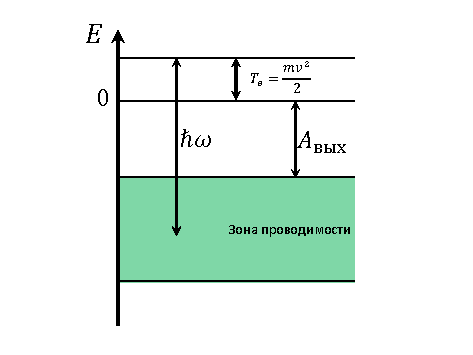
\includegraphics[width=0.6\textwidth,keepaspectratio]{Seminar_02/pics/pic_02.pdf}
    \caption{Структура уровней энергии для электронов в металле. За ноль принята энергия покоящегося свободного электрона.}
    \label{fig:sem_02_electron_energy}
\end{figure}

\subsection{Эффект Комптона}
В курсе оптики мы рассматривали классическое рэлеевское рассеяние на различных малых неоднородностях. Его основным физическим свойством было сохранение длины волны света при переизлучении его под углом. Однако, как я упоминал, есть множество других видов рассеяния, в частности --- комптоновское. В чем же оно заключается? Комптоновское рассеяние --- это рассеяние кванта света на свободном электроне с последующим уменьшением частоты. То есть, это, по своей сути, представляет задачу на упругое соударение безмассовой частицы света (фотона) и покоящегося электрона. И, так как при ударе электрон забирает часть энергии, то у фотона её становится меньше, и он <<краснеет>>. Как вы видите, здесь тоже применима гипотеза Планка о зависимости энергии фотонов от частоты.

\vspace{1em} \noindent
Давайте попробуем как-то это описать. Из классической электродинамики мы знаем о связи импульса и энергии фотона: $E = pc$ (стандартный опыт Лебедева с идеей о воздействии электромагнитного поля на электроны в атомах стенки). Поскольку мы хотим получить общее выражение для изменения длины волны, мы должны учитывать и возможные релятивистские эффекты. Из специальной теории относительности мы можем получить  один её из инвариантов для произвольной частицы: $E^2 -(pc)^2 = (mc^2)^2$. Этих двух вещей нам более чем достаточно, чтобы решить поставленную задачу об изменении длины волны фотона при рассеянии. У нее есть 2 возможных решения. Я расскажу оба, вы же решите для себя, что проще. Сама схема эксперимента представлена на рисунке \ref{fig:sem_02_kompton}.
\begin{figure}[h]
    \centering
    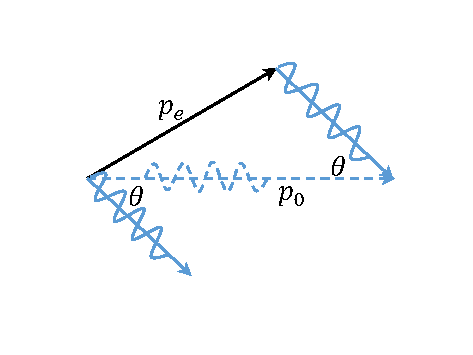
\includegraphics[width=0.5\textwidth,keepaspectratio]{Seminar_02/pics/pic_03.pdf}
    \caption{Рассеяние фотона на покоящемся электроне. Пунктирная линия -- импульс фотона до взаимодействия $p_0$.}
    \label{fig:sem_02_kompton}
\end{figure}

\paragraph{Классические формы законов сохранения}
Здесь мы запишем классическую систему из законов сохранения импульса и энергии, и решим ее, попутно воспользовавшись геометрией. Энергия и импульс фотона до столкновения --- $E_{ph0}$ $\textbf{p}_0$, после --- $E_{ph}$, $\textbf{p}$. Энергия и импульс электрона после столкновения $E_e$ $\textbf{p}_e$. Угол отклонения фотона $\theta$.
\begin{equation*}
    \left\{ 
    \begin{matrix}
        \textbf{p}_0 = \textbf{p}_e + \textbf{p}\\
        E_{ph0} + m_ec^2 = E_{ph} + E_e
    \end{matrix}
    \right\}
\end{equation*}
По теореме косинусов: 
\begin{equation*}
    p_e^2 = p_0^2 +p^2 - 2p_0p\cos{\theta}
\end{equation*}
Теперь попробуем получить аналогичную связь  из энергии с учетом инварианта СТО. Из второго уравнения выразим энергию электрона после удара и возведем в квадрат:
\begin{gather*}
    E_e = m_ec^2 + E_{ph0} - E_{ph}\\
    (m_ec^2)^2 + (p_ec)^2 = (m_ec^2) + E^2_{ph0} + E^2_{ph} - 2E_{ph0}E_{ph} - 2 m_ec^2(E_{ph} - E_{ph0})\\
    p_e^2 = p_0^2 +p^2 - 2(p_0p+m_ec(p-p_0))
\end{gather*}
Собирая вместе полученный результат и теорему косинусов, получаем:
\begin{equation}
\label{eq:sem_02_kompton}
    \Delta\lambda = \dfrac{h}{m_ec}(1-\cos{\theta}) = \lambdabar_c(1-\cos{\theta})
\end{equation}
Здесь $\lambdabar_c = 0.024$ нм --- комптоновская длина волны.

\vspace{1em} \noindent
В целом, метод кажется вполне рабочим, но в реальных задачах нам не всегда будет везти. Электрон может двигаться, например, или еще что похуже. Более того, тут еще нужно знать что делать, чтобы получить нужный результат. Дайте посмотрим альтернативынй метод.

\paragraph{Я у мамы теорфизик} Здесь я немного сошлюсь на ваши курсы теории поля, но, честно, это не будет больно. Во-первых, в теорфизе есть нотация 4-векторов для описания релятивистских частиц. Что это? Это просто вектор, состоящий из 4 компонент: на первом месте стоит энергия частицы, а со 2 по 4 --- компоненты обычного импульса частицы по координатам, умноженные на скорость света: $A = (E, p_xc, p_yc, p_zc)$. Во-вторых, квадрат такого вектора это не сумма квадратов всех компонент, а чуть более хитрая конструкция: $A^2 = E^2 -(p_x^2+p_y^2+p_z^2)c^2 = (mc^2)^2$, и она является нашим старым добрым СТО инвариантом. Также стоит отметить, что скалярное произведение двух 4-векторов меняется аналогичным квадрату образом: попарные произведения первых элементов идут с плюсом, остальные с минусом. Теперь сформулируем то же решение задачи на языке 4-векторов. Опустим компоненту z, так как всё происходит в плоскости, и получим:

\begin{gather*}
    \left( \begin{matrix}
    \hbar\omega_0\\
    \hbar\omega_0\\
    0\\
    \end{matrix}
    \right) + 
    \left( \begin{matrix}
    m_ec^2\\
    0\\
    0\\
    \end{matrix}
    \right) =
    \left( \begin{matrix}
    \hbar\omega\\
    \hbar\omega \cos{\theta}\\
    -\hbar\omega \sin{\theta}\\
    \end{matrix}
    \right) + 
    \left( \begin{matrix}
    E_e\\
    p_{ex}c\\
    p_{ey}c\\
    \end{matrix}
    \right)\\
    \\
        \left( \begin{matrix}
    \hbar\omega_0\\
    \hbar\omega_0\\
    0\\
    \end{matrix}
    \right) + 
    \left( \begin{matrix}
    m_ec^2\\
    0\\
    0\\
    \end{matrix}
    \right)
    +\left( \begin{matrix}
    -\hbar\omega\\
    -\hbar\omega \cos{\theta}\\
    \hbar\omega \sin{\theta}\\
    \end{matrix}
    \right)=
    \left( \begin{matrix}
    E_e\\
    p_{ex}c\\
    p_{ey}c\\
    \end{matrix}
    \right)
\end{gather*}
Теперь возведем левую и правую часть уравнений в квадрат, и воспользуемся его инвариантностью. Я специально запишу аккуратно, чтобы вам стало понятно, откуда что берется:
\begin{gather*}
    0+(m_ec^2)^2 + 0 + 2\hbar\omega_0 m_ec^2 - 2\hbar\omega m_ec^2- 2\hbar^2\omega_0\omega + 2\hbar^2\omega_0\omega\cos{\theta} = (m_ec^2)^2
\end{gather*}
После упрощения получим тот же результат (\ref{eq:sem_02_kompton}). Кажется, что этот вариант сложнее, но только потому, что он новый. В задачках с ним даже проще.

\vspace{1em} \noindent
Теперь несколько важных формул, которые нам понадобятся. Характерная кинетическая энергия электрона при комптновском рассеянии:
\begin{equation*}
    T_e = \hbar\omega_0 - \hbar\omega \approx \dfrac{hc}{\lambda^2}\Delta\lambda
\end{equation*}
Максимальная кинетическая энергия электрона при рассеянии фотона назад:
\begin{equation*}
    T_{max} =  \dfrac{hc}{\lambda^2}2\lambdabar_c = \dfrac{2E^2}{mc^2}
\end{equation*}
И последний комментарий о решенной нами задаче. Мы решили нечто более общее, чем просто рассеяние фотона на электроне. Абсолютно аналогично решается задача о рассеянии безмассовой частицы (например, нейтрино) на любой массивной частице.

\section{Практическая часть}
Часть задачек решаются практически подстановкой в формулы из теории. Я не буду скатываться до этого и порешаю что-то посложнее.

\subsection{Задача 1.17}

\label{task_117}
\paragraph{Условие} Какую минимальную длительность импульса фототока можно получить в вакуумном фотоэлементе, между анодом и катодом которого приложено напряжение в несколько сотен вольт, при освещении фотокатода короткими ($10^{-11}$ с) импульсами света с длиной волны $\lambda = 500$ нм? Красная граница материала фотокатода $\lambda_{\text{кр}} = 1000$ нм, напряженность поля между анодом и фотокатодом $E= 300$ В/см.

\paragraph{Решение} Давайте разберемся, с чего вдруг у импульса тока будет какая-то длительность, и почему она будет чем-то ограничена. Как я уже говорил в теоретической части, свет выбивает электроны не с фиксированной энергией, а электроны из зоны проводимости, такие, чтобы у них суммарно хватило энергии вылететь. И получается, что на выходе у нас есть целый спектр энергий электронов. Давайте разберемся с границами. Нижняя граница понятна --- это ноль (выбиваются самые <<глубокие>> электроны), а верхнюю границу по скорости и по энергии можно получить из закона Эйнштейна:
\begin{gather*}
    \dfrac{mV_{max}^2}{2} = \hbar(\omega - \omega_0) = hc\left(\dfrac{1}{\lambda} - \dfrac{1}{\lambda_0} \right)\\
    V^2_{max} = \dfrac{2hc}{m}\left(\dfrac{1}{\lambda} - \dfrac{1}{\lambda_0} \right)
\end{gather*}
Теперь у нас есть разбег начальной скорости электронов от 0 до $V_{max}$. И все они летят в поле ускоряющего напряжения $E$. Так у нас с вами осталась только кинематическая задачка о времени пролета наших электронов в трубке длиной $l$:
\begin{gather*}
    l = \dfrac{eEt_1^2}{2m} = V_{max}t_2 +\dfrac{eEt_2^2}{2m} \Rightarrow t_1 = t_2\sqrt{1+\dfrac{2mV_{max}}{eEt_2}}\\
    t_1 = t_2 + \dfrac{mV_{max}}{eE}
\end{gather*}
Здесь мы просто разложили этот корень с $t_2$, потому что значение добавки мало. Окончательно:
\begin{equation*}
    \Delta t = t_1 - t_2 = \dfrac{1}{eE}\sqrt{\dfrac{2hc}{m}\left(\dfrac{1}{\lambda} - \dfrac{1}{\lambda_0} \right)} = 1.2\cdot10^{-10} \text{с}
\end{equation*}

\subsection{Задача 1.32}
\label{task_132}
\paragraph{Условие} С какой скоростью $v$ должен двигаться электрон, чтобы летящий ему навстречу фотон с длиной волны $\lambda = 0,0024$ нм не изменил свою энергию при $180^\circ$-рассеянии?
\paragraph{Решение}
Здесь можно решить задачу через теорфизический метод, и я рекомендую ее вам сделать именно так, чтобы потренироваться, а сам покажу альтернативное решение, которое, возможно, проще.

\vspace{1em} \noindent
Запишем закон сохранения энергии с учетом релятивистской энергии электрона, где $\beta = v/c$:
\begin{equation*}
    \hbar\omega + \dfrac{mc^2}{\sqrt{1+\beta^2}}=\hbar\omega + \dfrac{mc^2}{\sqrt{1+\beta^{'2}}}
\end{equation*}
Единственным адекватным решением будет только то, где $\beta = \beta'$, то есть электрон летит с той же скоростью назад. Теперь запишем закон сохранение импульса:
\begin{gather*}
    \dfrac{\hbar\omega}{c} - \dfrac{mc\beta}{\sqrt{1+\beta^2}} = -\dfrac{\hbar\omega}{c} + \dfrac{mc\beta}{\sqrt{1+\beta^2}}\\
     \dfrac{mc\beta}{\sqrt{1+\beta^2}} = \dfrac{\hbar\omega}{c} = \dfrac{h}{\lambda}\\
     \dfrac{\beta}{\sqrt{1+\beta^2}} = \dfrac{h}{mc}\dfrac{1}{\lambda} = \dfrac{\lambdabar}{\lambda}\approx 1\\
\end{gather*}
Окончательно решаем уравнение на $\beta$ и находим, что $v = c/\sqrt{2}$.

\subsection{Задача 1.48}
\label{task_148}
\paragraph{Условие} Возбужденное ядро с энергией возбуждения $\Delta \epsilon = 1 $ МэВ с $A = 100$ движется с кинетической энергией $T = 100$ эВ и испускает $\gamma$-квант. Под каким углом к направлению движения ядра сдвиг $\gamma$-кванта по энергии будет равен нулю?

\paragraph{Решение} Что вообще происходит? У нас есть возбужденное ядро, которое летит с некоторой скоростью. Энергию возбуждения мы знаем. И вот оно решает скинуть возбуждение в виде гамма-кванта. Куда будет лететь этот квант? Куда угодно --- то есть под любым углом к первоначальному направлению движения ядра. А какую частоту этого гамма-кванта мы зафиксируем? Кажется очевидным, что $\hbar\omega = \Delta \epsilon$. Проблема в том, что это не так из-за эффекта Допплера. Напомню, что мы еще на первом курсе получили формулку сдвига частот, если источник движется со скоростью $v$:
\begin{equation*}
    \omega = \omega_0 \left(1+ \dfrac{v}{c}\cos{\theta} \right)
\end{equation*}
А поменялась частота --- поменяется и энергия. Так, первый фактор установили. Но при излучении гамма-кванта скорость у ядра тоже меняется, и, так как энергия гамма кванта высокая, то и изменение скорости существенное. Это тоже надо учесть. Для этого определим, сколько же энергии от возбуждения ушло в ядро. Воспользуемся тем, что импульсы ядра и гамма-кванта в системе покоя ядра одинаковые, и посчитаем этот сдвиг частот:
\begin{gather*}
    \Delta\omega = \dfrac{T_{new}}{\hbar} =  \dfrac{p^2}{2m\hbar} = \dfrac{E^_{\gamma}}{2mc^2\hbar}\\
    \omega = \dfrac{E_{\gamma} - T_{new}}{\hbar} = \dfrac{E_{\gamma}}{\hbar} \left(1-\dfrac{E^_{\gamma}}{2mc^2} \right)
\end{gather*}
С учетом этих двух сдвигов частот получаем:
\begin{equation*}
    \omega = \dfrac{E_{\gamma}}{\hbar} \left(1+ \dfrac{v}{c}\cos{\theta} - \dfrac{E^_{\gamma}}{2mc^2}\right)
\end{equation*}
И они должны скомпенсировать друг друга:
\begin{equation*}
    \dfrac{v}{c}\cos{\theta} = \dfrac{E^_{\gamma}}{2mc^2} \Rightarrow \cos{\theta} = \dfrac{E_\gamma}{v-2mc} = \dfrac{E_\gamma}{\sqrt{8Tmc^2}} \approx 0.116
\end{equation*}


\subsection{Комментарии к задачам из задания}
\paragraph{0-2-1} Зная мощность светового потока, можно спокойно найти импульс и удвоить его где нужно.
\paragraph{0-2-2} Подставить в формулу эффекта Комптона нужный угол.
\paragraph{Задача 1.7} Нужно вспомнить разложение амплитудной модуляции в спектр и посмотреть, кто выбивает электроны, а кто нет.
\paragraph{Задача 1.18} Нужно, как в первой неделе, прикинуть, сколько энергии приходит в атом, и посчитать, сколько времени займет накопление энергии на фотоэффект.
\paragraph{Задача 1.23} Нужно взять формулы из следствия уравнения Комптона.
\paragraph{Задача 1.35} Решить задачу на эффект Комптона, только с движущимся электроном.
\paragraph{Задача 1.39} Решена в задачнике.
\paragraph{Задача 1.48} Решена в \ref{task_148}.

\end{document}
